\usepackage{nccmath}

\begin{document}

%----------------------------------------------------------------------------------------
%	TITLE PAGE
%----------------------------------------------------------------------------------------

\title[Compression]{Talk 6: Compression in Federated Learning}
\date{2021-7-15}
\author[]{WEN Hao}

% \institute[北京航空航天大学] % Your institution as it will appear on the bottom of every slide, may be shorthand to save space
% {
% 数学科学学院 \\ % Your institution for the title page
% \medskip
% \textit{wenh06@gmail.com} % Your email address
% 北京航空航天大学 \\
% 数学科学学院 \qquad 北京航空航天大学
% }

% \logo{\includegraphics[height=1.5cm]{logo}}
% \logoii{\includegraphics[height=1cm]{logo2}}

% \date{\footnotesize 2021年4月13日} % Date, can be changed to a custom date

\setlength{\belowdisplayskip}{5pt} \setlength{\belowdisplayshortskip}{5pt}
\setlength{\abovedisplayskip}{5pt} \setlength{\abovedisplayshortskip}{5pt}

%------------------------------------------------

\begin{frame}
\titlepage % Print the title page as the first slide
\end{frame}

%------------------------------------------------
% Page 1

\begin{frame}
\frametitle{Compression in Federated Learning}

As is discussed previously (e.g. in the study of ``GADMM'' to ``CQ-GGADMM''), one of the main bottleneck {\color{red} communication cost} can be reduced using
\begin{itemize}
    \item compression
    \item {\pgfsetfillopacity{0.3}lazy aggregation (censoring)}
    \item {\pgfsetfillopacity{0.3}etc.}
\end{itemize}

\pause
\vspace{0.6em}

\pgfsetfillopacity{1}
The technique of compression mainly consists of
\begin{itemize}
    \item (randomized) quantization
    \item sparsification
\end{itemize}
or their combination.

\end{frame}

%------------------------------------------------

\section{Naive Compression Methods}

%------------------------------------------------
% Page 2

\begin{frame}
\frametitle{Deterministic Compression}

compression can be naively done via fixed reduction of precision (fixed bit of quantization) of parameters and/or gradients, e.g. {\color{red} half precision} (\texttt{float32} $\to$ \texttt{float16}) or {\color{red} mixed precision}.

\vspace{0.6em}

This is the common practice for acceleration of ordinary (non-distributed) model training process. e.g. the \href{https://pytorch.org/blog/accelerating-training-on-nvidia-gpus-with-pytorch-automatic-mixed-precision/}{PyTorch Post} on mixed precision training.

\end{frame}

%------------------------------------------------
% Page 3

\begin{frame}
\frametitle{TernGrad}

One extreme case of compression is to take the {\color{red}sign} of each coordinate of the stochastic gradient vector, which makes it binary (1-bit, $\pm 1$) or ternary ($\{-1, 0, +1\}$).

\vspace{0.8em}

\begin{columns}
\begin{column}{0.48\textwidth}
\begin{figure}
    \centering
    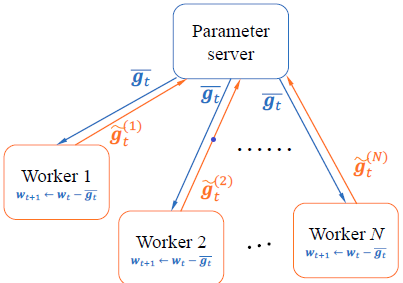
\includegraphics[width=1\textwidth,keepaspectratio]{images/terngrad.png}
\end{figure}
\end{column}
\begin{column}{0.48\textwidth}
$\widetilde{g}_t^{(i)}$ is the {\color{red}ternarized} gradient given by
$$g_t^{(i)} = \lVert g_t^{(i)} \rVert_{\infty} \cdot \operatorname{sign}(g_t^{(i)}) \odot \framebox{\color{red} $b_t$}$$
where $b_t$ is a random binary vector satisfying some Bernoulli distribution $Be(\lvert g_{t,k}^{(i)} \rvert / s_t)$
\end{column}
\end{columns}

\vspace{0.8em}

Similar algorithms include 1-bit SGD \cite{seide2014_1bitsgd}, signSGD \cite{bernstein2018signsgd}

\end{frame}

%------------------------------------------------
% Page 3

\begin{frame}
\frametitle{QSGD}

More generally, in QSGD \cite{alistarh2017qsgd}, randomized quantization (called ``low-precision quantizer'' in \cite{khirirat2018dcgd}) is performed on gradients $v$ via
$$Q_s(v) = \lVert v \rVert_2 \cdot \operatorname{sign}(v) \odot \framebox{\color{red}$\xi(v,s)$},$$
where the $i$-th element in vector $\xi(v,s)$ is defined by
\begin{equation*}
    \xi_i(v,s) = \begin{cases}
    (\ell+1)/s, & \text{with prob. } (|v_i|/\lVert v \rVert_2) s - \ell \\
    \ell/s, & \text{otherwise}
    \end{cases}
\end{equation*}
$s$ controls the number of quantization levels, and $\ell$ ({\color{red} should be $\ell_i$?}) be s.t. $|v_i|/\lVert v \rVert_2 \in [\ell/s, (\ell+1)/s]$.

\end{frame}

%------------------------------------------------
% Page 3

\begin{frame}
\frametitle{DCGD}

DCGD \cite{khirirat2018dcgd} generalized such operators $Q_s$ into an abstract concept

\begin{Def}[Unbiased Random Quantizer (URQ)]
A mapping $Q:\mathbb{R}^d \to \mathbb{R}^d$ is called an unbiased random quantizer if $\forall v \in \mathbb{R}^d$,
\begin{itemize}
    \item $\operatorname{supp}(Q(v)) \subseteq \operatorname{supp}(v)$
    \item $\expectation [Q(v)] = v$
    \item $\expectation [\lVert Q(v) \rVert_2^2] \leqslant \alpha \lVert v \rVert_2^2$ for some finite positive $\alpha$
\end{itemize}
\end{Def}

And perhaps with more useful properties like
\begin{itemize}
    \item sparsity: $\expectation [\lVert Q(v) \rVert_0] \leqslant$ const
    \item sign preserving: $Q(v)_i \cdot v_i \geqslant 0$
\end{itemize}

\end{frame}

%------------------------------------------------
% Page 3

\begin{frame}
\frametitle{Examples of URQs}

Despite the ternary quantizer and low-precision quantizer, one has \cite{lizhize2020adiana}

\only<1>{
\begin{block}{Random-$k$ sparsification}
$$\mathcal{C}(v) = \dfrac{d}{k} (v \odot \xi_k)$$
where $\xi_k \in \{0, 1\}^d$ is a uniformly random binary vector with $k$ nonzero entries, $v \in \mathbb{R}^d$.
\end{block}
}

\only<2>{
\begin{block}{$(p,s)$-quantization}
$$\mathcal{C}_{p,s}(v) = \operatorname{sign}(v)\cdot \lVert v \rVert_p \cdot \dfrac{1}{s} \xi(v,s)$$
where $\xi(v,s)$ is a random vector with i-th element
\begin{equation*}
\xi_i(v,s) = \begin{cases}
\ell_i+1, & \text{with prob. } (|v_i|/\lVert v \rVert_2) s - \ell_i \\
\ell_i, & \text{otherwise}
\end{cases}
\end{equation*}
and $\ell_i$ be s.t. $|v_i|/\lVert v \rVert_2 \in [\ell/s, (\ell+1)/s]$
\end{block}
}

\end{frame}

%------------------------------------------------
% Page 3

\begin{frame}
\frametitle{Compressors (Quantizers)}

One can refer to \href{https://github.com/burlachenkok/marina}{https://github.com/burlachenkok/marina} for code and examples of various compressors, e.g. in files
\begin{itemize}
    \item \href{https://github.com/burlachenkok/marina/blob/main/linear_model_with_non_convex_loss/compressors.py}{linear\_model\_with\_non\_convex\_loss/compressors.py}
    \item \href{https://github.com/burlachenkok/marina/blob/main/neural_nets_experiments/compressors.py}{neural\_nets\_experiments/compressors.py}
\end{itemize}

\vspace{0.8em}

or \href{https://github.com/wenh06/fl_seminar/blob/master/code/compressors_test.ipynb}{this simple jupyter notebook}

\end{frame}

%------------------------------------------------

\section{Recent Development}

%------------------------------------------------
% Page 3

\begin{frame}
\frametitle{(A)DIANA}

The main contribution of (A)DIANA \cite{mishchenko2019diana,lizhize2020adiana} is that, instead of quantizing the gradients, the {\color{red} difference of gradient updates}, i.e. instead of
$$\widetilde{g}^{(i)}_t = Q(g^{(i)}_t) = Q(\nabla f_i(x_t))$$
one performs
\begin{equation*}
    \begin{cases}
    \widetilde{g}^{(i)}_t = \widetilde{h}^{(i)}_t + Q(\colorbox{pink}{$\nabla f_i(x_t) - h^{(i)}_t$}) \\
    \colorbox{pink}{$h^{(i)}_{t+1} = h^{(i)}_t + \alpha Q(\nabla f_i(x_t) - h^{(i)}_t)$}
    \end{cases}
\end{equation*}

$h^{(i)}$ are ``memory'' maintained locally, whose average is maintained in the central server.

\end{frame}

%------------------------------------------------
% Page 3

\begin{frame}
\frametitle{(A)DIANA}

Another key point (feature) of (A)DIANA is the combination with acceleration (and variance reduction):

\only<1>{
\begin{figure}
    \centering
    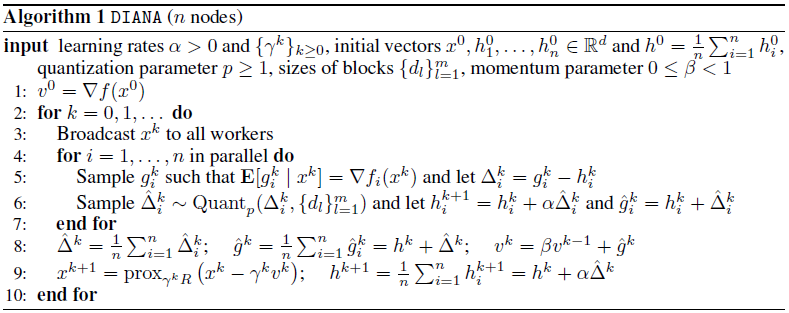
\includegraphics[width=0.9\textwidth,keepaspectratio]{images/diana.png}
\end{figure}

{\footnotesize Note the ``Quant'' operator is a so-called ``block-quantizer'' or ``bucket-quantizer''\cite{alistarh2017qsgd}}
}
\only<2>{
\begin{figure}
    \centering
    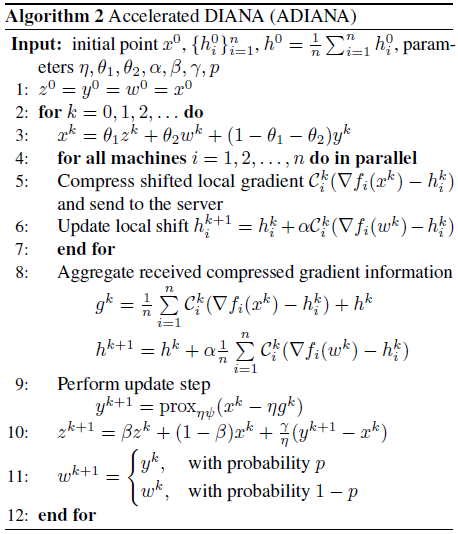
\includegraphics[width=0.54\textwidth,keepaspectratio]{images/adiana.png}
\end{figure}
}

\end{frame}

%------------------------------------------------
% Page 3

\begin{frame}
\frametitle{MARINA}

MARINA \cite{gorbunov2021marina} replaced the unbiased compressor by a {\color{red}biased} one, via replacing
\begin{equation*}
\begin{cases}
\widetilde{g}^{(i)}_t = \widetilde{h}^{(i)}_t + Q(\nabla f_i(x_t) - h^{(i)}_t) \\
h^{(i)}_{t+1} = h^{(i)}_t + \alpha Q(\nabla f_i(x_t) - h^{(i)}_t)
\end{cases}
\end{equation*}
by
\begin{equation*}
\widetilde{g}^{(i)}_t = 
\begin{cases}
\nabla f_i(x_t), & \text{with prob. } p \\
\widetilde{g}^{(i)}_{t-1} + Q(\nabla f_i(x_t) - \nabla f_i(x_{t-1})), & \text{with prob. } 1-p
\end{cases}
\end{equation*}
for some small $p$.

\pause
\vspace{0.6em}

As claimed by the authors, their intuition come from the rare (?) phenomenon in stochastic optimization that
\begin{quote}
`` the bias of the stochastic gradient helps to achieve better complexity''
\end{quote}

\end{frame}

%------------------------------------------------
% Page 3

\begin{frame}
\frametitle{MARINA}

The basic MARINA algorithm is as follows:

\begin{figure}
    \centering
    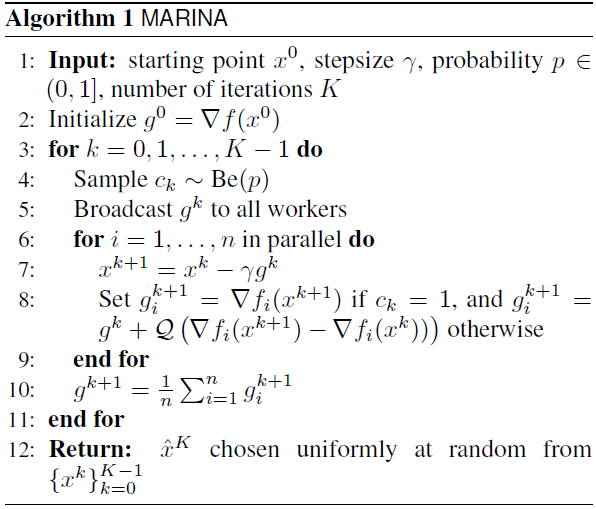
\includegraphics[width=0.7\textwidth,keepaspectratio]{images/marina.png}
\end{figure}

\end{frame}

%------------------------------------------------
% Page 3

\begin{frame}
\frametitle{More?}

\begin{itemize}
    \item higher order methods \cite{crane2019dingo,islamov2021distributed}
    \item combination with lazy aggregation \cite{issaid2020cq-ggadmm}, and with stochastic update
    \item biased compression \cite{beznosikov2020biased,safaryan2020uncertainty}
    \item analysis of communication cost (\# rounds and bandwidth)
\end{itemize}

\pause
\vspace{0.6em}

and more, to be continued...

\end{frame}

%------------------------------------------------
% Page 3

\begin{frame}
\frametitle{Additional resources from FLOW}

\begin{itemize}
    \item \href{https://sites.google.com/view/one-world-seminar-series-flow/archive/2021\#h.x17wddrti6j0}{MARINA: Faster Non-Convex Distributed Learning with Compression}
    \vspace{1em}
    \item \href{https://sites.google.com/view/one-world-seminar-series-flow/archive/2020\#h.5y43fcudf8t}{On Biased Compression for Distributed Learning}
\end{itemize}

\end{frame}

%------------------------------------------------
% Page 15

\begin{frame}[allowframebreaks]
\frametitle{References}

{\footnotesize
\bibliographystyle{ieeetr}
\bibliography{references}
}

\end{frame}

%------------------------------------------------

\end{document}
